%! alt Two concentric circles with centre O and radii 16 and 39, with A on the inner circle and B on the outer. At the moment contact begins, angle AOB is 120 degrees and AB = 49. Segment AB just touches the disc of radius r around O, at the foot F of the perpendicular from O, with a right angle at F.
%! after_paragraph 7
%! scale 2/17
% The shared preamble of every Kyuclid figure. pipeline/figures turns these colours into theme-aware paint,
% and refuses any other colour, so draw only with them:
%   figink (lines and labels), figaux (construction lines), figaccent (the object the argument turns on),
%   figtint and figaccenttint (light fills).
\documentclass[border=1.5pt]{standalone}
\usepackage{tkz-euclide}
\definecolor{figink}{RGB}{0,0,0}
\definecolor{figaux}{RGB}{85,85,85}
\definecolor{figaccent}{RGB}{192,57,43}
\definecolor{figtint}{RGB}{221,221,221}
\definecolor{figaccenttint}{RGB}{245,213,208}
% tkz-euclide's defaults draw circles, compasses and marks in 50% grey and fill points with a tint.
\makeatletter
\def\tkz@otherlinecolor{figink}
\def\tkz@euc@circlecolor{figink}
\def\tkz@euc@compasscolor{figink}
\def\tkz@euc@mkcolor{figink}
\def\tkz@mk@fill{figink}
\def\tkz@euc@pointfillcolor{figink}
\makeatother
\tkzSetUpLine[color=figink,line width=.7pt]
\tkzSetUpArc[color=figink,line width=.7pt]
\tkzSetUpCompass[color=figink,line width=.5pt]
\tkzSetUpPoint[color=figink,fill=figink,size=3.1pt]
\tikzset{
  every picture/.style={line cap=round,line join=round,color=figink},
  circle style/.append style={color=figink,line width=.7pt},
  aux/.style={color=figaux,line width=.45pt,dash pattern=on 2.6pt off 2pt},
  key/.style={color=figaccent,line width=1pt},
  mk/.style={color=figink,line width=.5pt},
  lbl/.style={color=figink,inner sep=2.2pt},
  len/.style={color=figink,inner sep=1.5pt,font=\small},
}

\begin{document}
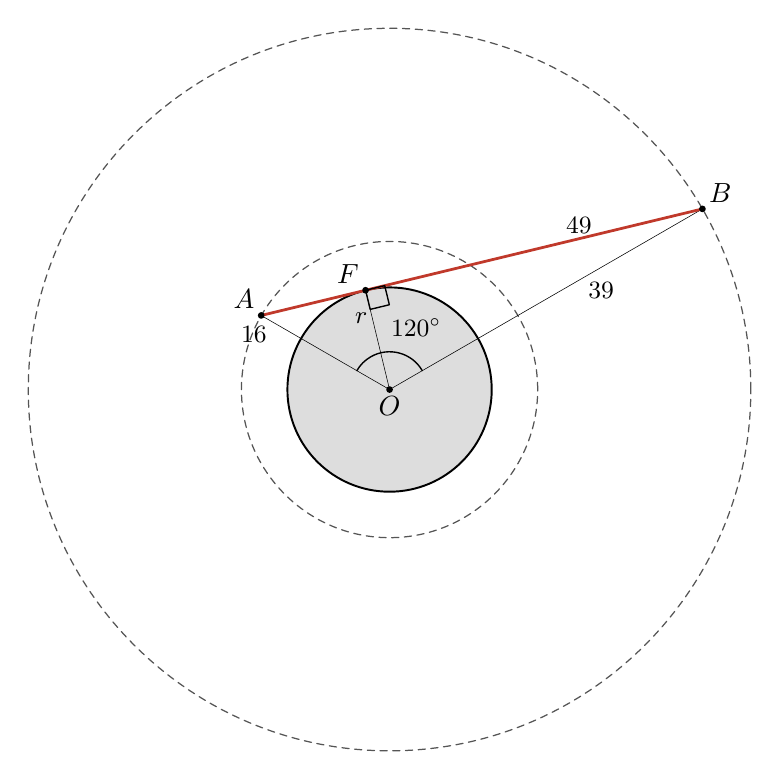
\begin{tikzpicture}
%! let r = 312*sqrt(3)/49
\tkzDefPoint(0.0,0.0){O} %! O = (0, 0)
\tkzDefPoint(-1.6301655,0.94117647){A} %! A = polar(O, 16, 150)
\tkzDefPoint(3.9735283,2.2941176){B} %! B = polar(O, 39, 30)
\tkzDefPoint(-0.30451029,1.2612392){F} %! F = foot(O, A, B)
\tkzDefPoint(2.2941176,-3.9735283){E} %! E = polar(O, 39, 300)
%! fact dist(O, A) == 16
%! fact dist(O, B) == 39
%! fact angle(A, O, B) == 120
%! fact dist(A, B) == 49
%! fact on_segment(F, A, B)
%! fact tangent(O, r, A, B)
%! fact dist(O, F) == r
%! fact perp(O, F, A, B)
\tkzFillCircle[color=figtint](O,F)
\tkzDrawCircle[aux](O,E)
\tkzDrawCircle[aux](O,A)
\tkzDrawCircle(O,F)
\tkzDrawSegments(O,A O,B)
\tkzDrawSegment[key](A,B)
\tkzDrawSegment(O,F)
\tkzMarkRightAngle[size=.25,mk](O,F,B)
\tkzMarkAngle[size=.48,arc=l,mark=none,mk](B,O,A)
\tkzDrawPoints(O,A,B,F)
\tkzLabelPoint[above left,lbl](A){$A$}
\tkzLabelPoint[above right,lbl](B){$B$}
\tkzLabelPoint[below,lbl](O){$O$}
\tkzLabelPoint[above left,lbl](F){$F$}
\tkzLabelSegment[below left,pos=.92,len](O,A){$16$}
\tkzLabelSegment[below right,pos=.62,len](O,B){$39$}
\tkzLabelSegment[left,pos=.72,len](O,F){$r$}
\tkzLabelAngle[pos=.86,font=\small](B,O,F){$120^\circ$}
\tkzLabelSegment[above,pos=.72,len](A,B){$49$}
\end{tikzpicture}
\end{document}
